\chapter{Ensayos y resultados experimentales}

\section{Introducción}

Una vez implementado el sistema de control diseñado en la placa de desarrollo Nexys 3, se realizan una serie de ensayos para verificar su correcto funcionamiento. Estos ensayos son de carácter progresivo, en un principio probando sólamente al generador de la señal PWM junto con el ADC en un esquema lazo abierto. Luego de ir confirmando el correcto funcionamiento, se fueron agregando más componentes al sistema para finalmente realizar un ensayo con el lazo cerrado de tensión.

Con el algoritmo de control completo, se arman diferentes tipos de configuraciones con el sistema híbrido eléctrico, con el objetivo de probar distintas topologías del sistema híbrido eléctrico y observar sus características.

Si bien el proyecto se encuentra orientado al uso de baterías de litio, todos los ensayos preliminares fueron realizados utilizando una fuente de potencia emulando el comportamiento de las baterías. Esto se debió a cuestiones de seguridad tanto de la electrónica utilizada como de los usuarios, ya que tratándose de una estación de ensayo experimental aún resta incorporar elementos de seguridad para las baterías, de las cuales la fuente de potencia ya presenta algunas (como limitación de corriente). 



\section{Con fuente de potencia}

Las primeras pruebas realizadas a lazo abierto consistieron en la utilización del controlador PWM para las señales de los transistores del convertidor CC-CC. Luego, se implementó al controlador del conversor analógico-digital para permitir la variación del ciclo de trabajo mediante un potenciómetro, cuyo valor era filtrado por el filtro diseñado e implementado a \SI{1.5}{\kilo\hertz}.

En estos ensayos iniciales fue utilizada la fuente de potencia para poder probar al algoritmo implementado en la FPGA en un ambiente controlado, en el caso de algún error tanto en el diseño como en la programación.

\subsection{Lazo de control de corriente}

El primer ensayo a lazo cerrado consistió en el control de la corriente por el inductor del convertidor CC-CC. En este sistema fueron utilizados los componentes ya probados anteriormente: el controlador PWM; el controlador del ADC; y el filtro de corriente de \SI{1.5}{\kilo\hertz}. Para poder cerrar el lazo, se incorporaron dos nuevos elementos: la referencia de corriente; y el controlador PI, para poder calcular la acción de control que permita a la corriente de entrada seguir a la referencia.

Como medida de seguridad, se implementaron llaves que permiten habilitar o deshabilitar al integrador del controlador. Además, este componente posee una saturación a su salida, para evitar la obtención de un ciclo de trabajo mayor a 1 o 100\%; y el método anti-windup explicado anteriormente.

En primera instancia, las pruebas realizadas con el algoritmo de control de corriente consistieron únicamente en el componente proporcional del controlador. Al realizar pequeños escalones de \SI{0.5}{\ampere}, se corroboró que el sistema a lazo cerrado reaccionaba acordemente a estos saltos, pero con un error de estado estacionario significativo, como era de esperarse al estar deshabilitada la parte integral del controlador. Una vez activado el integrador, se pudo observar cómo la corriente de inductor seguía a la referencia impuesta por el FPGA sin error de estado estacionario.

Luego de haber verificado el correcto comportamiento del sistema de control de corriente, se realizaron una serie de ensayos sucesivos que permitieron realizar un ajuste fino de los parámetros del controlador PI para lograr una mejor performance del algoritmo, que además permita un tiempo de establecimiento rápido con un sobrepico de corriente aceptable.

Realizando escalones de \SI{3}{\ampere} con el sistema de control ajustado, se obtuvieron los resultados de la Figura \ref{escalones-lazo-corriente}. Se puede observar que la corriente se establece en el nuevo valor de referencia en cuestión de microsegundos sin causar un sobrepico abrupto o peligroso, y por lo tanto se considera que el lazo de corriente controla satisfactoramiente a la variable de estado. Estas formas de onda fueron obtenidas directamente desde el osciloscopio. A su vez se encuentran superpuestas las curvas de simulacion, que permiten validar la metodología de diseño de los parámetros del controlador PI.

\begin{figure}[hbt!]
  \centering
  \subfloat[Escalón negativo de \SI{3}{\ampere}.]{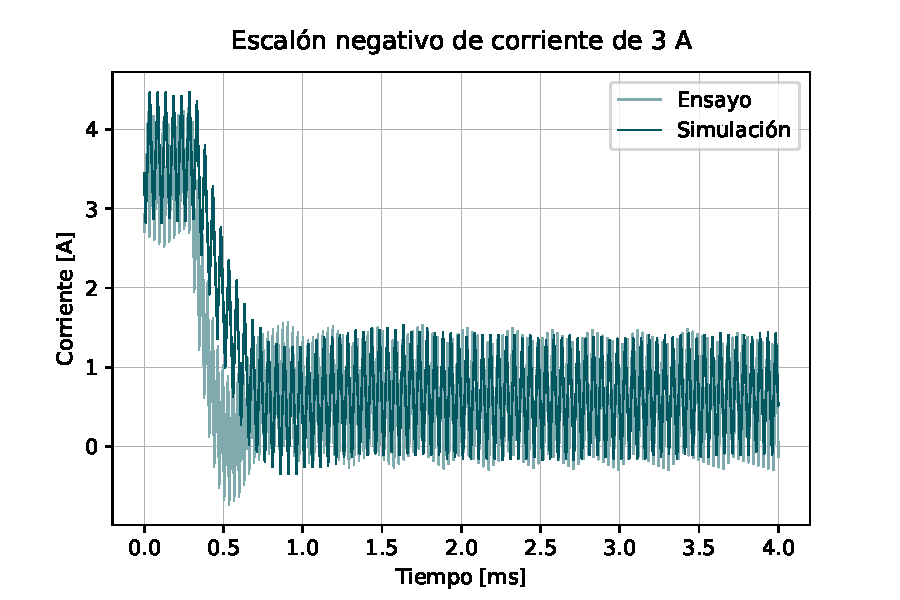
\includegraphics[width=0.45\textwidth]{Imágenes/Ensayos/Con fuente de potencia/Lazo interno de corriente/Fuente de potencia/Escalón negativo de corriente.pdf}}    
  \subfloat[Escalón positivo de \SI{3}{\ampere}.]{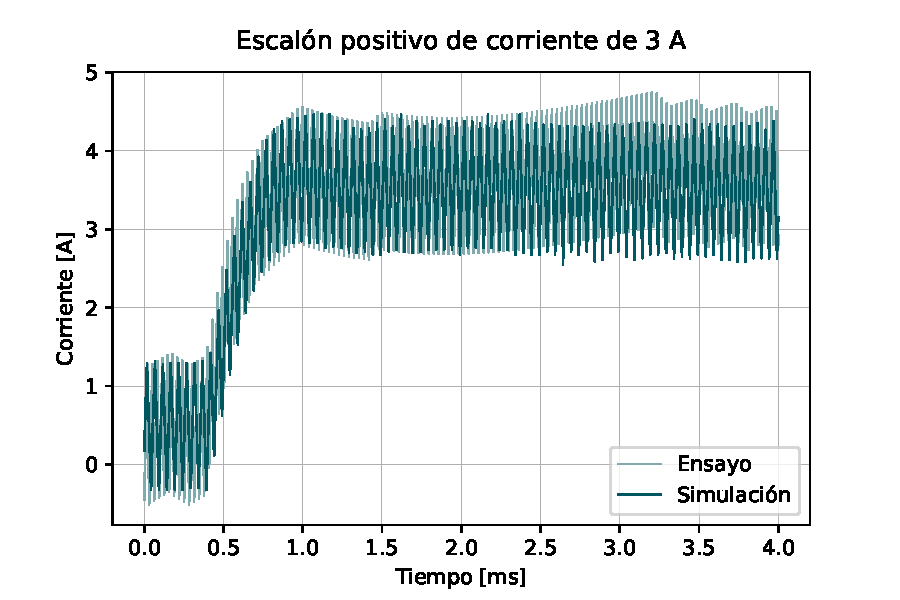
\includegraphics[width=0.45\textwidth]{Imágenes/Ensayos/Con fuente de potencia/Lazo interno de corriente/Fuente de potencia/Escalón positivo de corriente.pdf}}
  \caption{Resultados de los ensayos del lazo de corriente.}
  \label{escalones-lazo-corriente}
\end{figure}

\subsection{Lazo de control de tensión}

Para el lazo de control de tensión se realizaron una serie de ensayos bajo distintas condiciones para determinar la performance del sistema de control implementado. Los primeros ensayos consistieron en pequeños escalones en la tensión de referencia de \SI{1}{\volt}. Al observar el valor de tensión de carga con el sistema de control implementado, era posible percibir una variación de este en los dígitos menos significativos de los display de la placa de desarrollo (potencialmente producto del ripple de tensión de carga más ruido presente en el sistema), lo cual llevó a la implementación de un filtro digital para su medición mediante el conversor analógico-digital. Debido a las características de VHDL (explicadas en capítulos anteriores), la implementación de este filtro consistió únicamente en la instanciación del componente utilizado para el filtrado de la corriente de entrada.

\begin{figure}[hbt!]
  \centering
  \subfloat[Escalón negativo de \SI{40}{\ohm} a \SI{20}{\ohm}.]{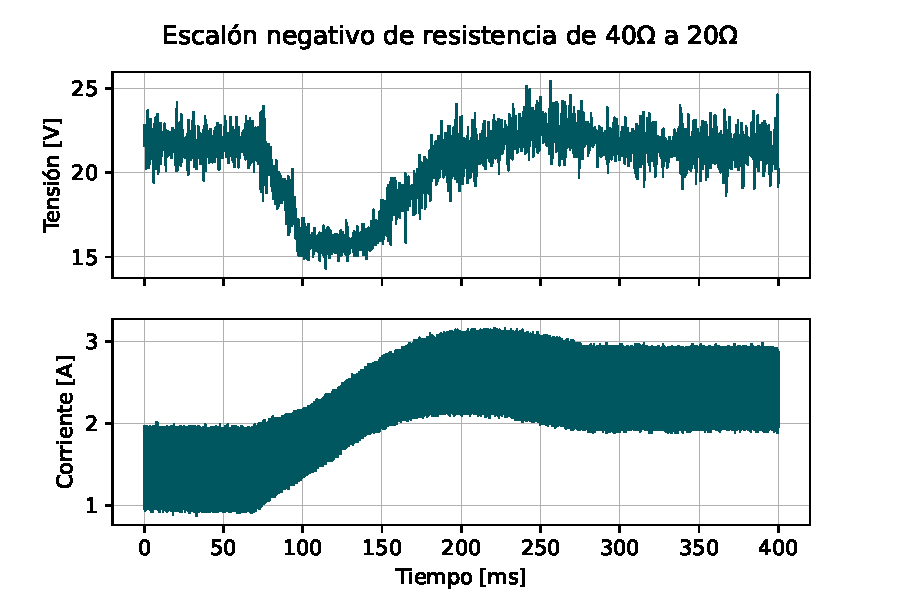
\includegraphics[width=0.45\textwidth]{Imágenes/Ensayos/Con fuente de potencia/Lazo externo de tensión/Escalón negativo de resistencia.pdf}}    
  \subfloat[Escalón positivo de \SI{20}{\ohm} a \SI{40}{\ohm}.]{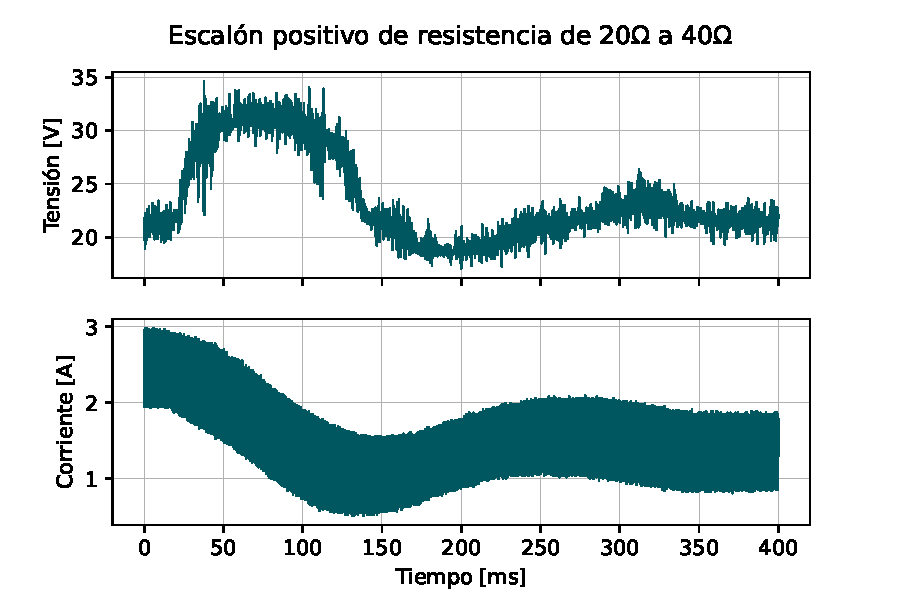
\includegraphics[width=0.45\textwidth]{Imágenes/Ensayos/Con fuente de potencia/Lazo externo de tensión/Escalón positivo de resistencia.pdf}}
  \caption{Resultados de los ensayos del lazo de tensión.}
  \label{var-r-lazo-tension}
\end{figure}

Una vez verificado el correcto funcionamiento del sistema a lazo cerrado, se realizaron pruebas más demandantes al lazo de control, variando la resistencia de carga y observando la respuesta de la corriente de entrada y tensión de salida. En la Figura \ref{var-r-lazo-tension} pueden observarse las respuestas de ambas variables de estado para un salto de \SI{20}{\ohm} a \SI{40}{\ohm} con una referencia impuesta en \SI{24}{\volt}. En ambos casos puede observarse una rápida y robusta recuperación del nivel de tensión establecido por la referencia. Para el caso del escalón positivo de resistencia, existe una leve oscilación que termina en el establecimiento de la tensión de salida en un valor de \SI{24}{\volt}.



\section{Con supercapacitores}

Con el algoritmo de control completo probado mediante la fuente de potencia, se incorpora al banco de supercapacitores, construido en el instituto por parte del Ing. Fornaro, como elemento extra del sistema, y se realizan otra serie de ensayos para observar su comportamiento bajo distintos tipos de situaciones.

\subsection{Supercapacitores del lado de baja tensión}
\label{sc-como-alimentacion}

La primer configuración ensayada con los supercapacitores fue colocando al banco en el lado de baja tensión del convertidor, en paralelo con la fuente principal del sistema. El esquema propuesto que representa a la topología usada para esta serie de ensayos puede observarse en la Figura \ref{esquema-sc-fuente}.

\begin{figure}[hbt!]
  \centering
  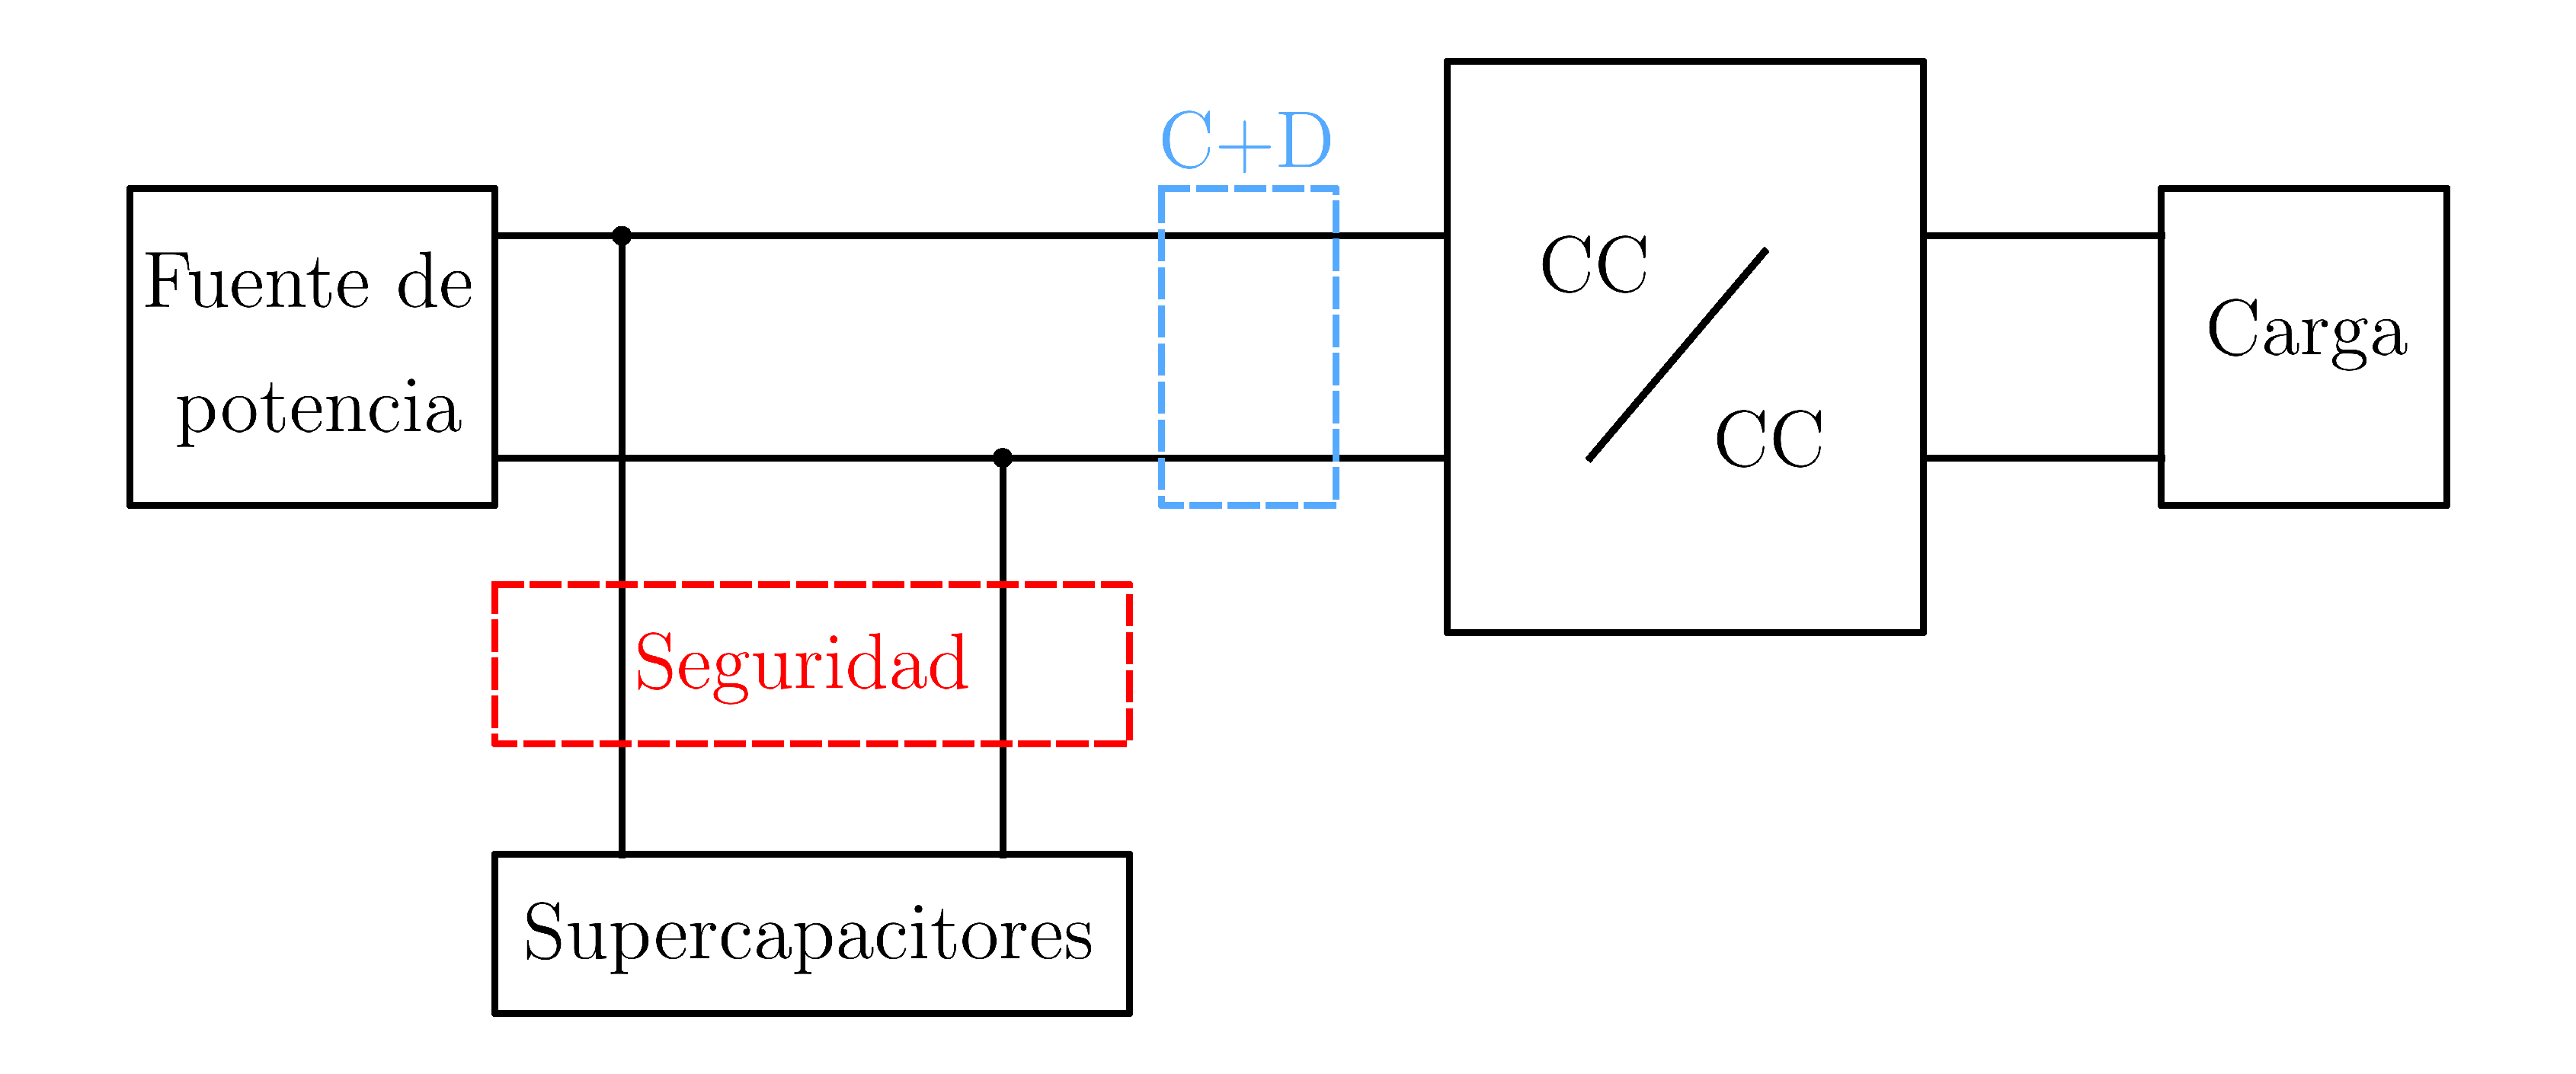
\includegraphics[width=0.80\columnwidth]{Imágenes/Ensayos/Con módulos de almacenamiento/Supercapacitores/Como fuente/Diagrama del ensayo.pdf}
  \caption{Diagrama del sistema con el banco de supercapacitores como fuente de energía.}
  \label{esquema-sc-fuente}
\end{figure}

Esta topología permite al banco de supercapacitores entregar picos de demanda y el rizado de corriente del convertidor, mientras que la fuente de potencia suministra la potencia media necesitada.

En el sistema también se encuentran el módulo de seguridad del banco de supercapacitores, implementado por el Ing. Riva; un banco de capacitores; y finalmente un par de diodos en antiparalelo con el convertidor CC-CC, que permiten un camino seguro para la corriente en el caso de que se produzca una apertura del circuito de supercapacitores debido a la acción del módulo de seguridad.

\subsubsection{Sin inductor}

Los ensayos realizados con el banco de supercapacitores en el lado de baja tensión consistieron en la observación de la tensión de carga, la corriente de los supercapacitores, y la corriente de la fuente de potencia al generar una variación de la resistencia de carga. Con un salto negativo de resistencia de \SI{40}{\ohm} a \SI{20}{\ohm} y uno positivo de \SI{20}{\ohm} a \SI{40}{\ohm}, se obtuvieron las formas de onda de la Figura \ref{sc-fuente}:

\begin{figure}[hbt!]
  \centering
  \subfloat[Escalón negativo de \SI{40}{\ohm} a \SI{20}{\ohm}.\label{sc-fuente-40-20-ohm}]{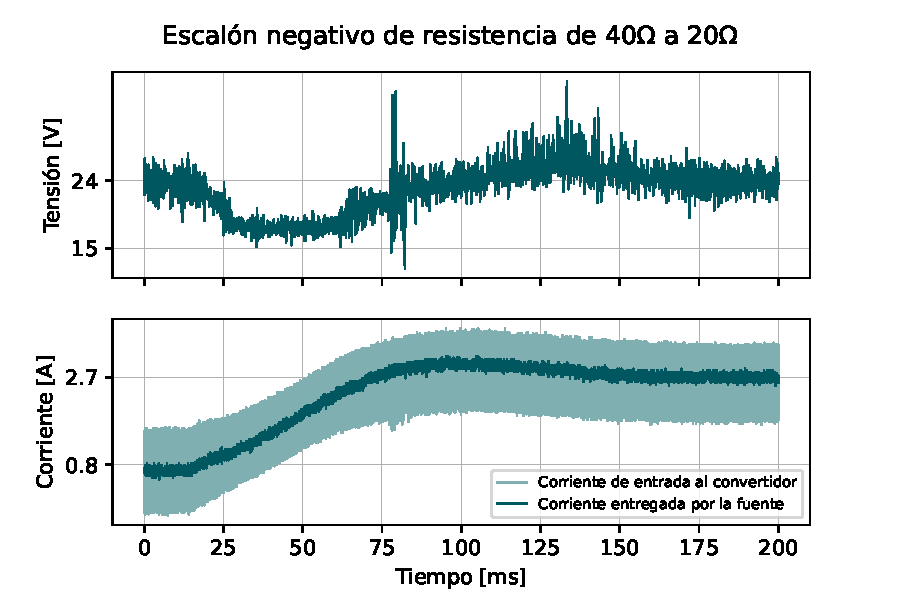
\includegraphics[width=0.45\textwidth]{Imágenes/Ensayos/Con módulos de almacenamiento/Supercapacitores/Como fuente/Sin inductor/Escalón negativo de resistencia.pdf}}    
  \subfloat[Escalón positivo de \SI{20}{\ohm} a \SI{40}{\ohm}.\label{sc-fuente-20-40-ohm}]{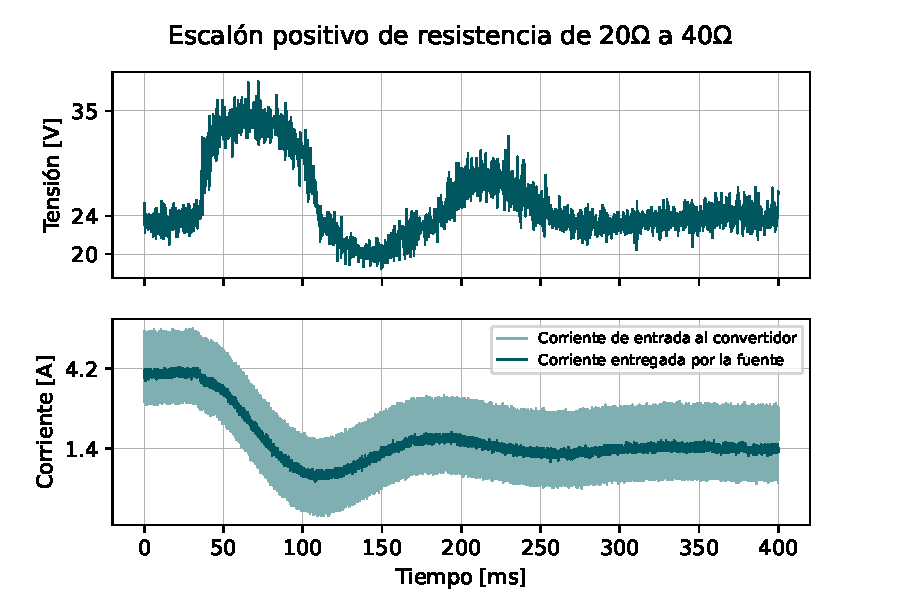
\includegraphics[width=0.45\textwidth]{Imágenes/Ensayos/Con módulos de almacenamiento/Supercapacitores/Como fuente/Sin inductor/Escalón positivo de resistencia.pdf}}
  \caption{Tensión de carga y corrientes con un variación de resistencia de carga.}
  \label{sc-fuente}
\end{figure}

En ambos casos es posible observar cómo la corriente media es entregada por la fuente, mientras que el banco de supercapacitores únicamente suministra al ripple de corriente del convertidor. Por lo tanto, la premisa (la cual era que los supercapacitores suministraban la potencia en un pico de demanda) por la que fue construida esta topología es parcialmente cumplida. Esto puede deberse a que la fuente de potencia posee una dinámica lo suficientemente rápida para cubrir el pico de demanda para el ensayo realizado. Bajo este pretexto, se coloca un inductor entre la fuente de potencia y el banco de supercapacitores, de modo de generar un dinámica interna que emule a una fuente de energía no ideal.

\subsubsection{Con inductor}

Colocado un inductor de \SI{2000}{\micro\henry} entre la fuente y el banco, se proceden a realizar los mismos ensayos mencionados anteriormente. En la Figura \ref{sc-fuente-40-20-ohm-inductor} pueden observarse las formas de onda obtenidas para un escalón negativo de resistencia de \SI{40}{\ohm} a \SI{20}{\ohm}, mientras que la tensión y las corrientes para el escalón positivo se encuentran en la Figura \ref{sc-fuente-20-40-ohm-inductor}.

\begin{figure}[hbt!]
  \centering
  \subfloat[Escalón negativo de \SI{40}{\ohm} a \SI{20}{\ohm}.\label{sc-fuente-40-20-ohm-inductor}]{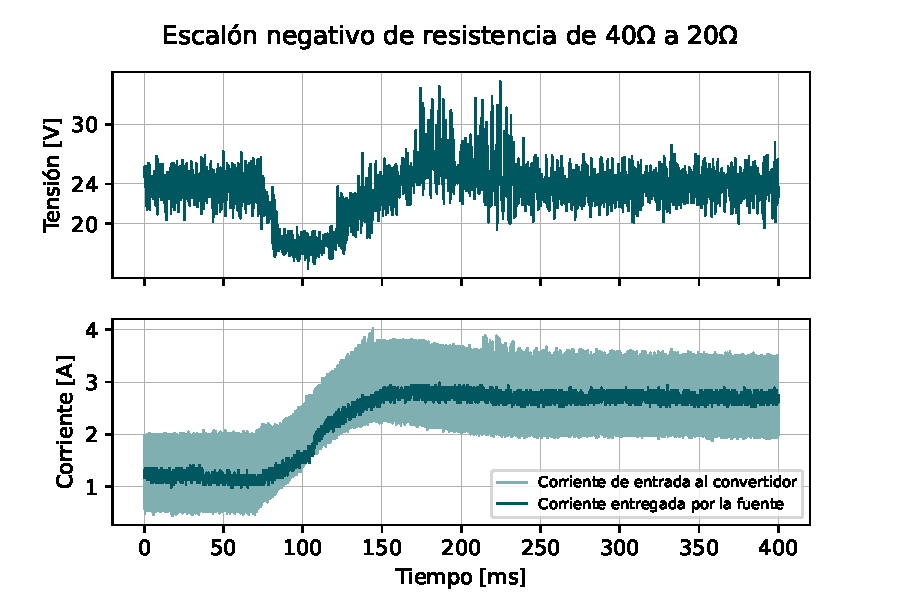
\includegraphics[width=0.45\textwidth]{Imágenes/Ensayos/Con módulos de almacenamiento/Supercapacitores/Como fuente/Con inductor/Escalón negativo de resistencia.pdf}}    
  \subfloat[Escalón positivo de \SI{20}{\ohm} a \SI{40}{\ohm}.\label{sc-fuente-20-40-ohm-inductor}]{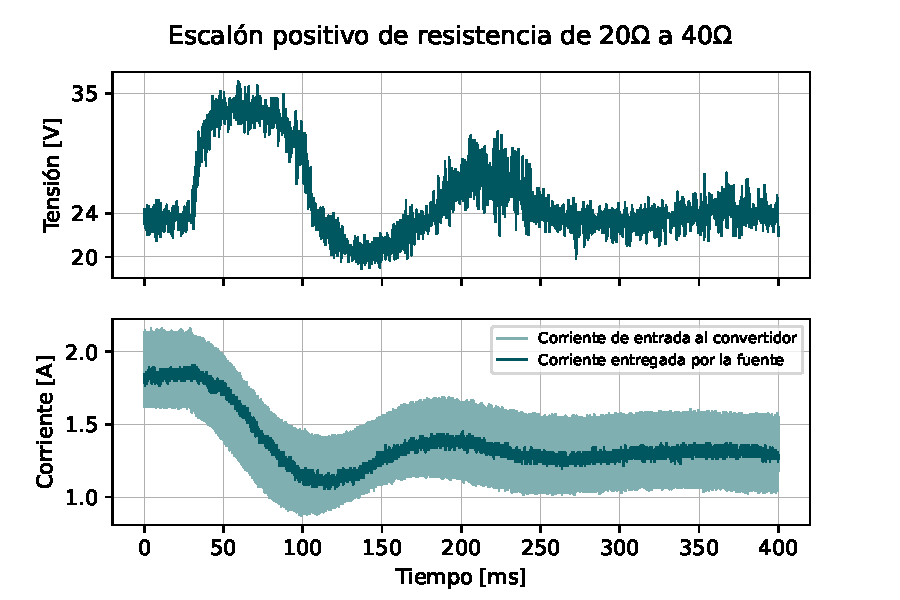
\includegraphics[width=0.45\textwidth]{Imágenes/Ensayos/Con módulos de almacenamiento/Supercapacitores/Como fuente/Con inductor/Escalón positivo de resistencia.pdf}}
  \caption{Tensión de carga y corrientes con un variación de resistencia de carga.}
  \label{sc-fuente-inductor}
\end{figure}

En estos ensayos, y especialmente el de la Figura \ref{sc-fuente-40-20-ohm-inductor}, es claramente visible el comportamiento esperado para esta topología. Puede observarse cómo la corriente del banco de supercapacitores presenta una dinámica notablemente más rápida que la de la fuente de potencia con el inductor, y por lo tanto es la que proveé la demanda inicial provocada por el escalón de resistencia de carga. Después de un tiempo, ambas corrientes se establecen en el mismo valor medio.

Para el escalón positivo de resistencia de carga se presenta el mismo comportamiento del sistema, pero de forma menos acentuada.

\subsection{Supercapacitores del lado de la carga}

La siguiente configuración ensayada fue con el banco de supercapacitores en el bus de continua como carga. Esta topología se presenta en la Figura \ref{esquema-sc-carga}.

\begin{figure}[hbt!]
  \centering
  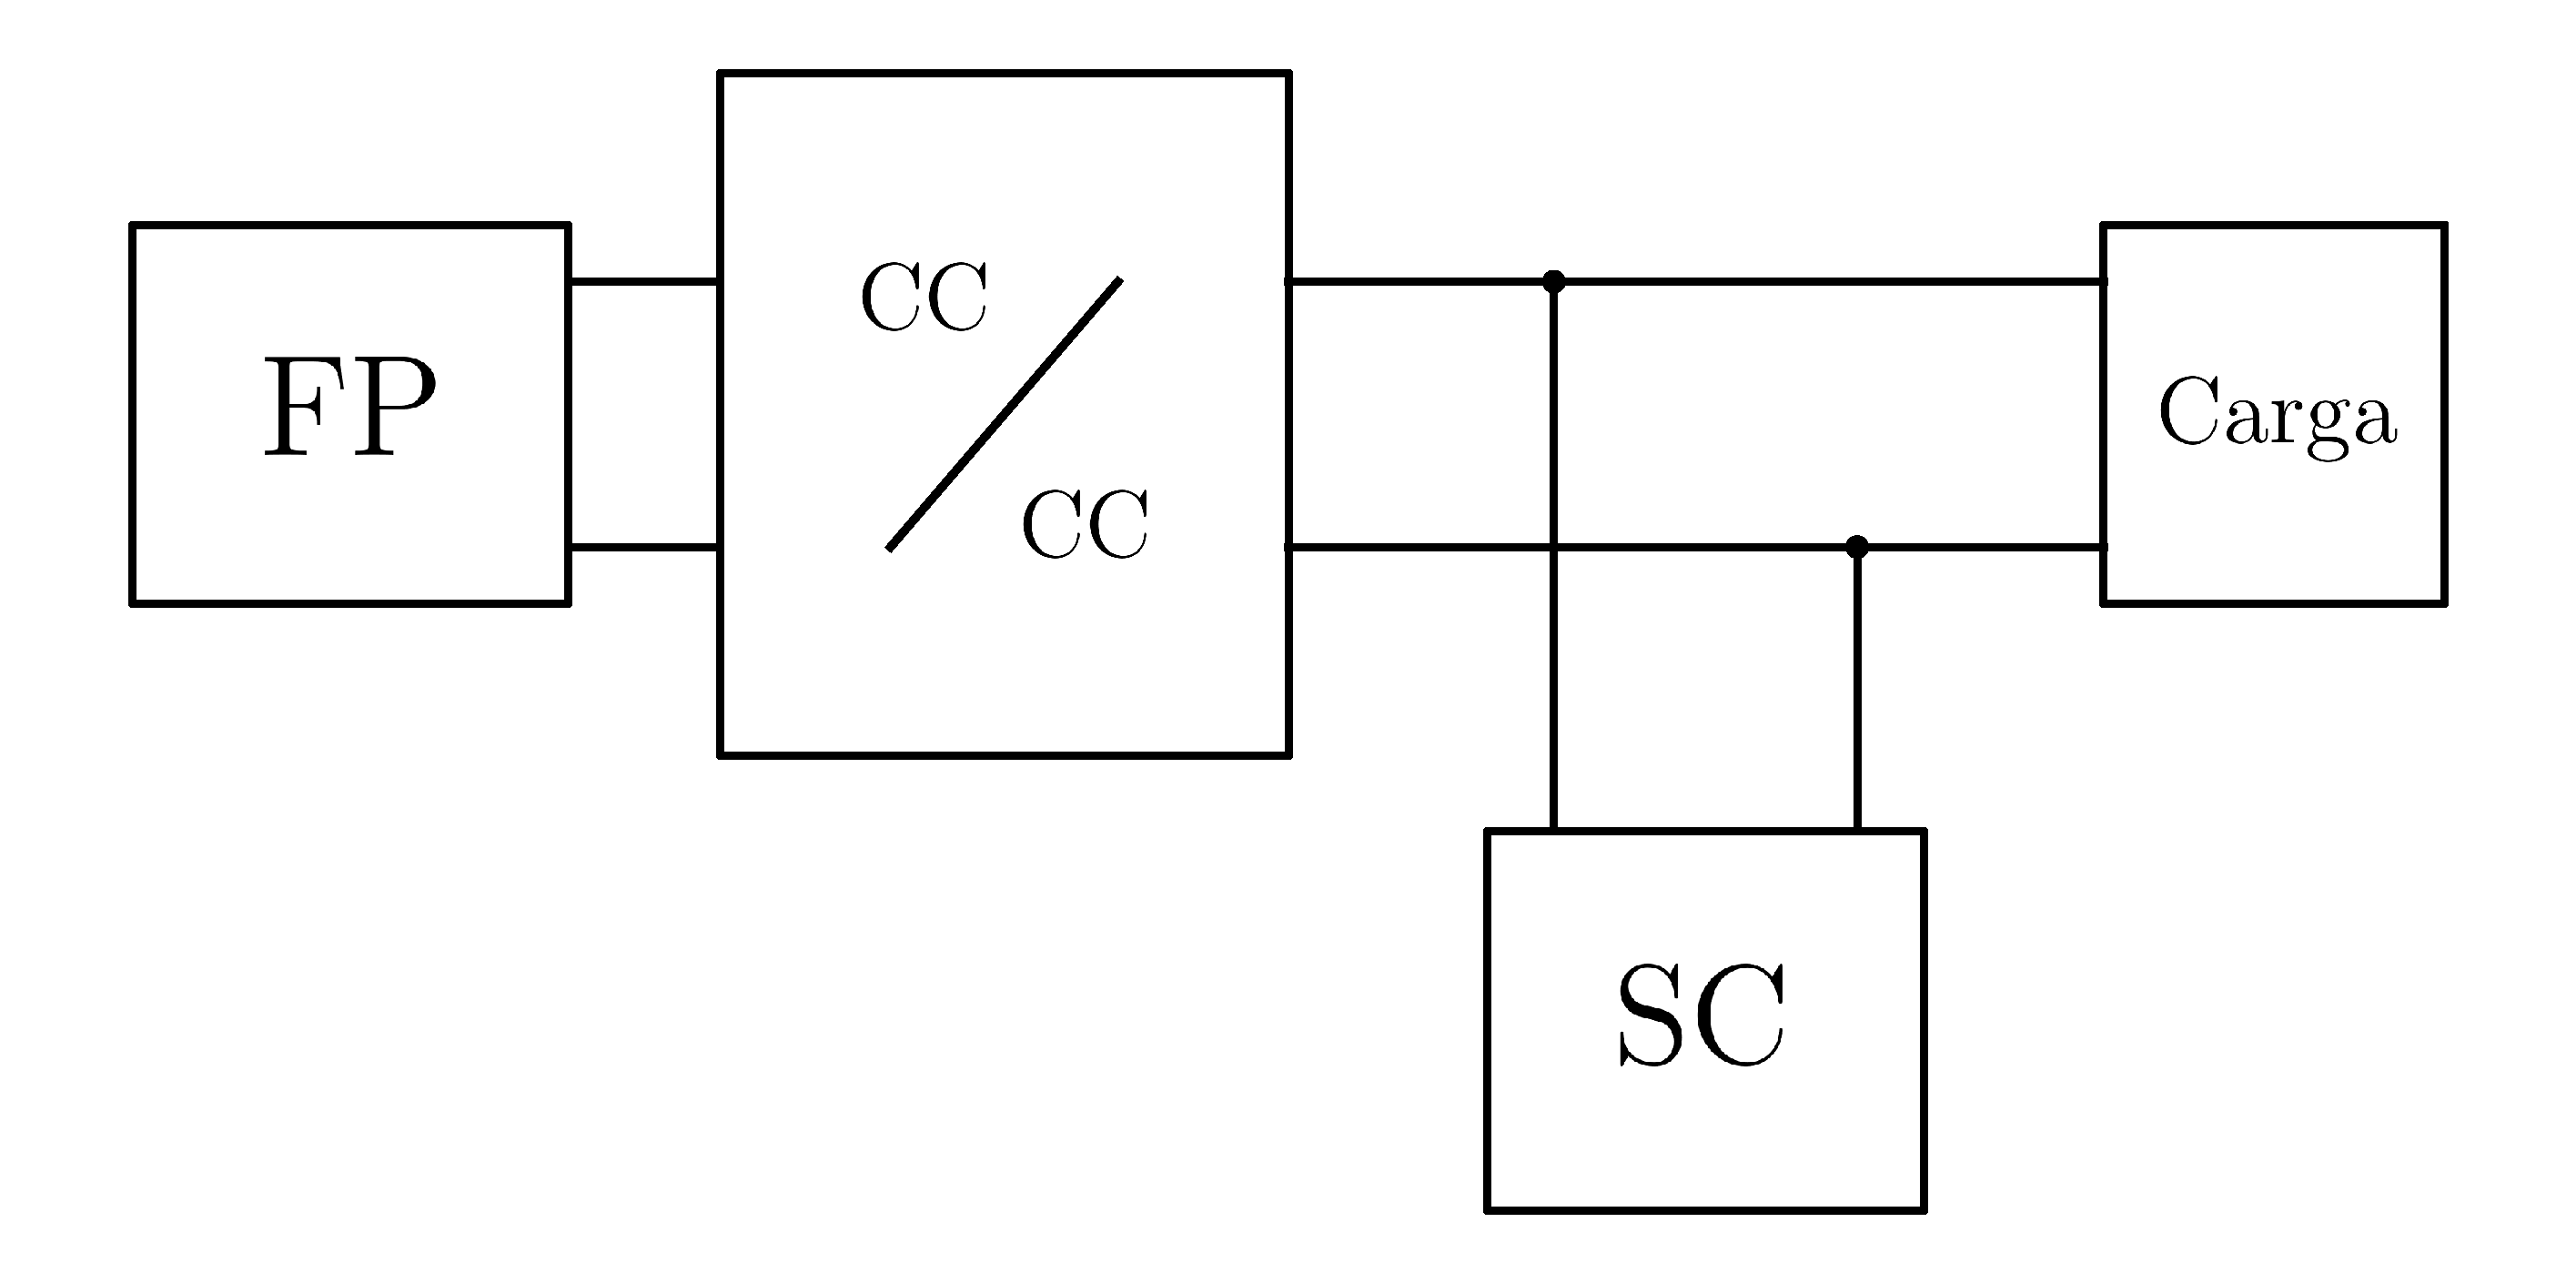
\includegraphics[width=0.55\columnwidth]{Imágenes/Ensayos/Con módulos de almacenamiento/Supercapacitores/Como carga/Diagrama del ensayo.pdf}
  \caption{Diagrama del sistema con el banco de supercapacitores como carga.}
  \label{esquema-sc-carga}
\end{figure}

Esta configuración permite la conexión del banco directamente con la carga. Debido a la gran capacitancia presentada por el banco de supercapacitores, las pruebas hechas presentan una dinámica lenta respecto a los ensayos anteriores (del orden de decenas de minutos), y como es inversamente proporcional a la derivada de la tensión de carga, es necesario aumentar la velocidad del controlador PI de tensión para ajustarse a esta nueva dinámica. Mediante una simulación a través de Simulink\textsuperscript\textregistered\hspace{0.6pt}, se establecieron unas nuevas constantes proporcional e integral que se ajustan a la dinámica del sistema.

Debido a que el osciloscopio es incapaz de capturar formas de onda con tal período de tiempo, fue utilizada la comunicación UART implementada en la placa de desarrollo. En la Figura \ref{sc-carga} se observan las formas de onda resultantes.

\begin{figure}[hbt!]
  \centering
  \subfloat[Corriente por el inductor.\label{sc-carga-i-carga}]{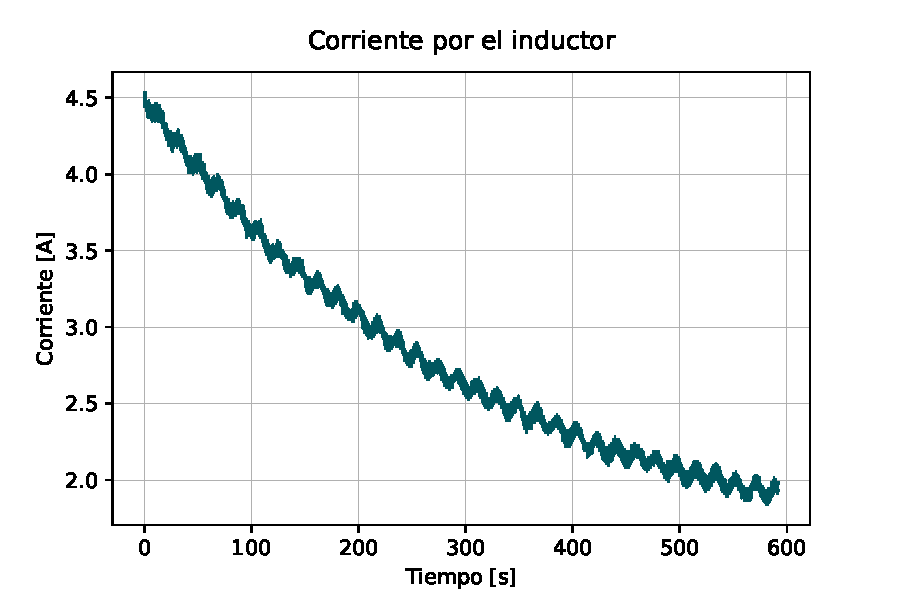
\includegraphics[width=0.45\textwidth]{Imágenes/Ensayos/Con módulos de almacenamiento/Supercapacitores/Como carga/Carga de supercapacitores/Corriente por el inductor.pdf}}    
  \hspace{3.5mm}
  \subfloat[Tensión en la carga.\label{sc-carga-v-carga}]{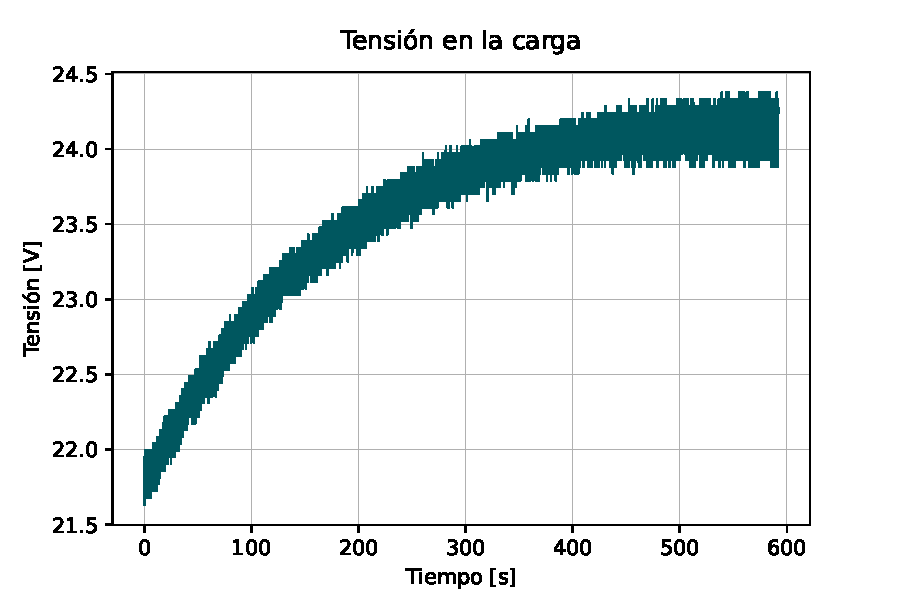
\includegraphics[width=0.45\textwidth]{Imágenes/Ensayos/Con módulos de almacenamiento/Supercapacitores/Como carga/Carga de supercapacitores/Tensión en la carga.pdf}}
  \hspace{3.5mm}
  \subfloat[Acción de control de tensión.\label{sc-carga-u_u-carga}]{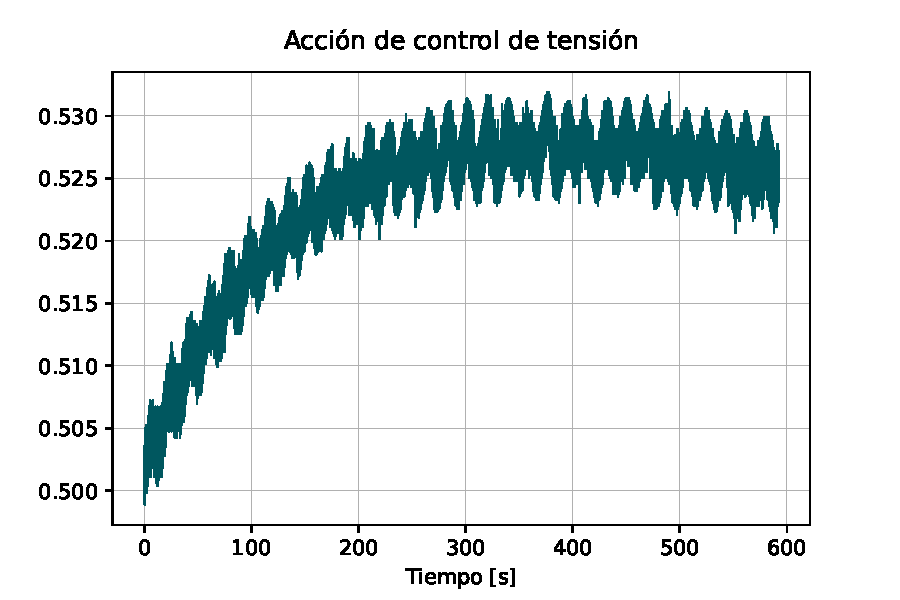
\includegraphics[width=0.45\textwidth]{Imágenes/Ensayos/Con módulos de almacenamiento/Supercapacitores/Como carga/Carga de supercapacitores/Control de tensión.pdf}}
  \hspace{3.5mm}
  \subfloat[Acción de control de corriente.\label{sc-carga-u_i-carga}]{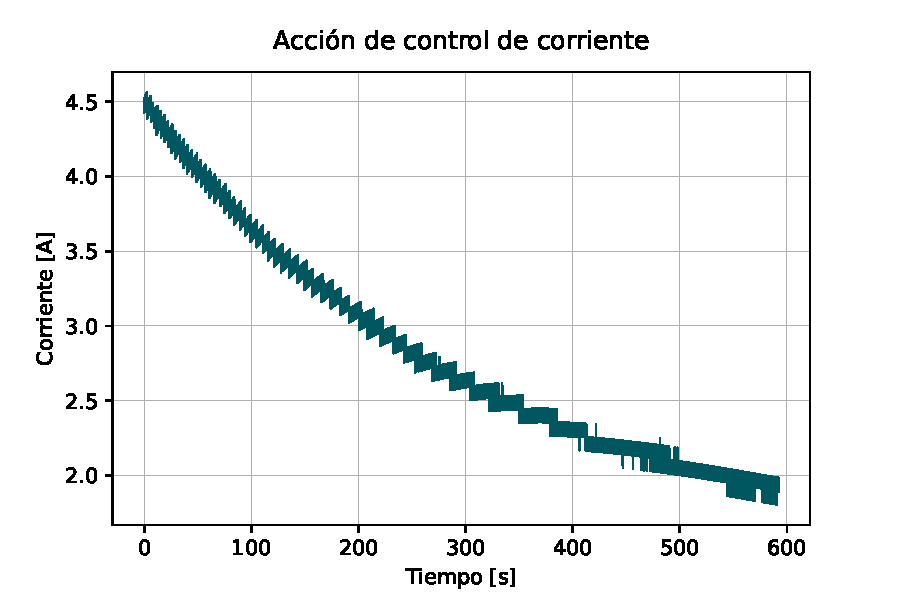
\includegraphics[width=0.45\textwidth]{Imágenes/Ensayos/Con módulos de almacenamiento/Supercapacitores/Como carga/Carga de supercapacitores/Control de corriente.pdf}}
  \caption{Formas de onda obtenidas en la simulación del lazo de control de corriente.}
  \label{sc-carga}
\end{figure}

Estableciendo la referencia en \SI{24}{\volt}, se observa en el proceso de carga del banco cómo la corriente de inductor disminuye mientras la tensión del banco se va acercando a la tensión de referencia, y cómo esta corriente refleja a la acción de control del lazo externo de tensión, el cual genera la referencia de corriente. A su vez, la acción de control del lazo interno de corriente aumenta mientras se carga el banco de supercapacitores, de modo de mantener la tensión del banco constante.

En el eje horizontal se puede observar la magnitud de decenas de minutos que posee este proceso de carga y por lo cual fueron necesarios ajustar los parámetros de los controladores PI de tal manera de que su velocidad de cálculo sea acorde con la dinámica del sistema.

Una vez completamente cargado el banco de supercapacitores, se realizan saltos de resistencia de carga y se registran la tensión y corrientes resultantes mediante la transmisión por UART. En la Figura~\ref{sc-carga-20-40-ohm} se grafican las formas de onda con un escalón positivo de resistencia, nuevamente de \SI{20}{\ohm} a \SI{40}{\ohm}.

En este ensayo se observa cómo en un lapso aproximado de 13 minutos, en el cual la tensión de carga presenta un leve sobrepico de aproximadamente \SI{600}{\milli\volt} para después establecerse en la tensión de referencia de \SI{24}{\volt}. Para el caso de la corriente de inductor se presenta una forma de onda próxima a una respuesta amortiguada.

\begin{figure}[hbt!]
  \centering
  \subfloat[Corriente por el inductor.\label{sc-carga-i-20-40-ohm}]{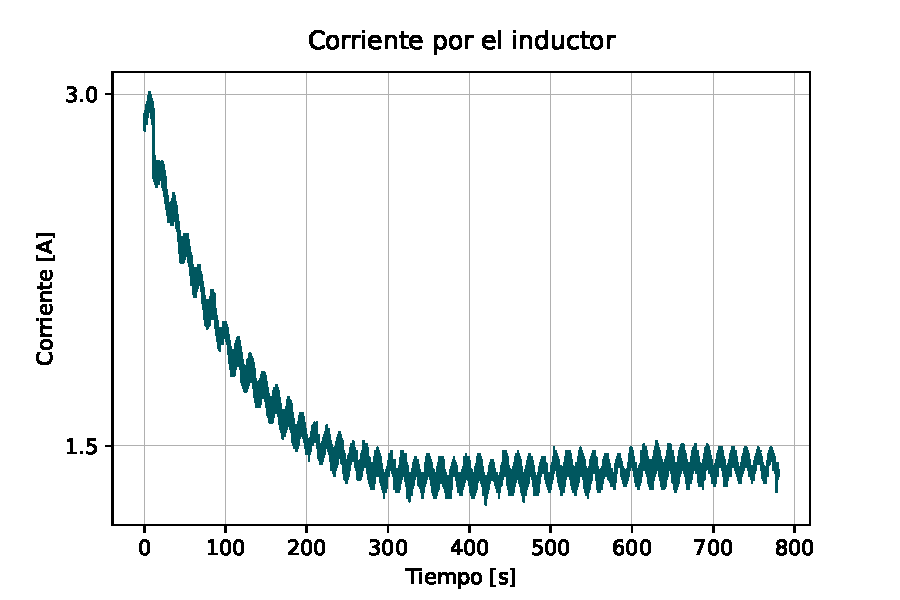
\includegraphics[width=0.45\textwidth]{Imágenes/Ensayos/Con módulos de almacenamiento/Supercapacitores/Como carga/Escalón positivo de resistencia/Corriente por el inductor.pdf}}    
  \hspace{3.5mm}
  \subfloat[Tensión en la carga.\label{sc-carga-v-20-40-ohm}]{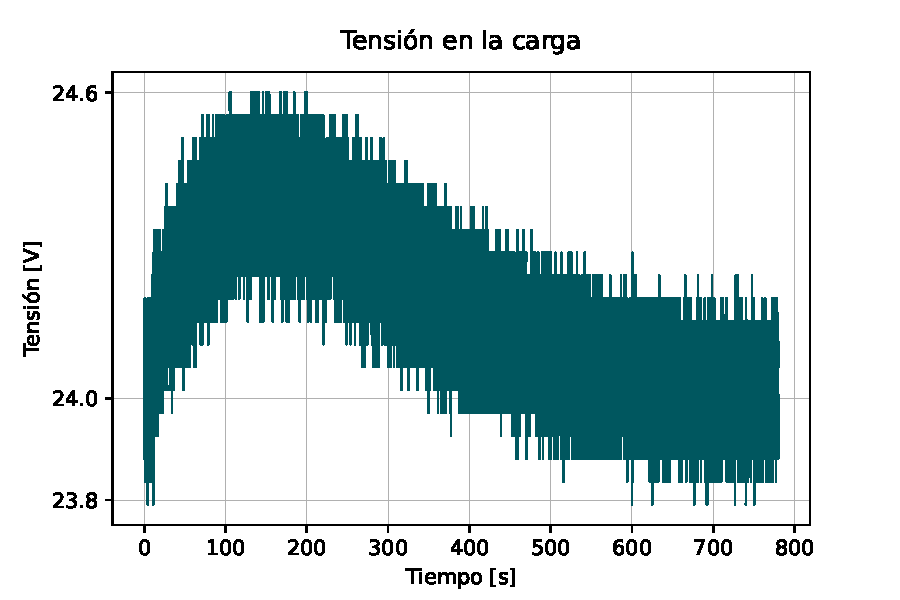
\includegraphics[width=0.45\textwidth]{Imágenes/Ensayos/Con módulos de almacenamiento/Supercapacitores/Como carga/Escalón positivo de resistencia/Tensión en la carga.pdf}}
  \hspace{3.5mm}
  \subfloat[Acción de control de tensión.\label{sc-carga-u_u-20-40-ohm}]{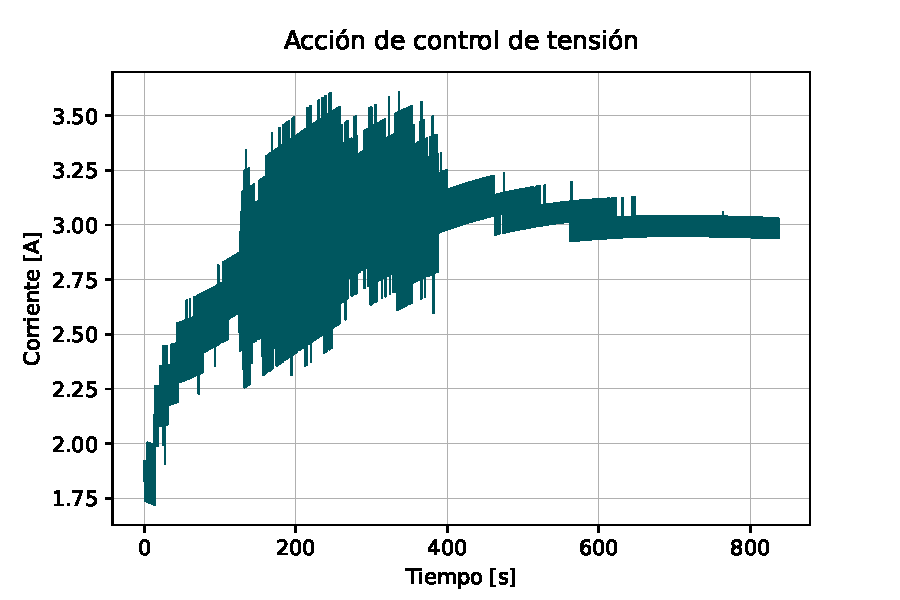
\includegraphics[width=0.45\textwidth]{Imágenes/Ensayos/Con módulos de almacenamiento/Supercapacitores/Como carga/Escalón positivo de resistencia/Control de tensión.pdf}}
  \hspace{3.5mm}
  \subfloat[Acción de control de corriente.\label{sc-carga-u_i-20-40-ohm}]{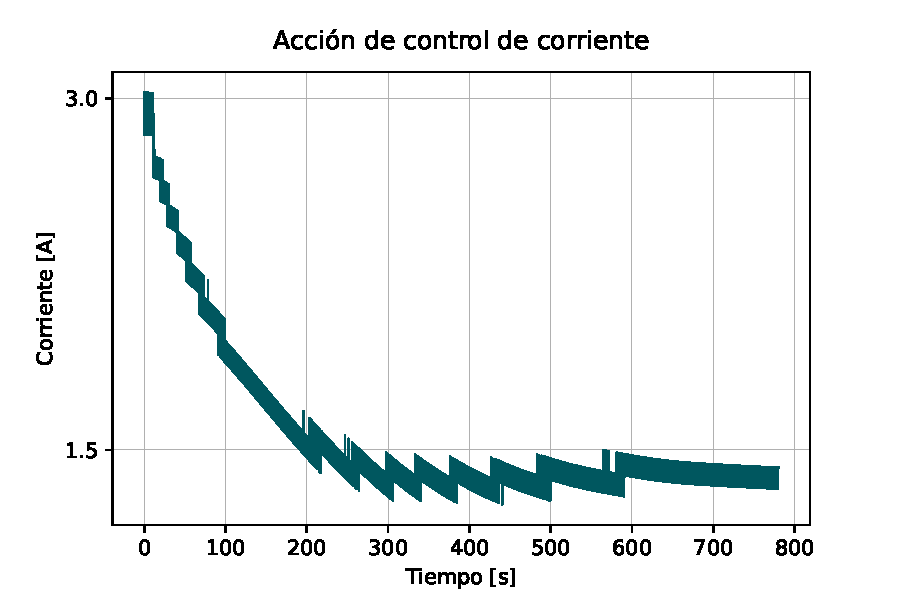
\includegraphics[width=0.45\textwidth]{Imágenes/Ensayos/Con módulos de almacenamiento/Supercapacitores/Como carga/Escalón positivo de resistencia/Control de corriente.pdf}}
  \caption{Formas de onda obtenidas con un salto positivo de resistencia.}
  \label{sc-carga-20-40-ohm}
\end{figure}

\section{Con fuente de potencia y supercapacitores}

La última configuración del sistema híbrido ensayada fue combinando ambos supercapacitores y fuente de potencia, haciendo uso de los dos convertidores CC-CC en el instituto. Esta topología se presenta en la Figura \ref{esquema-fp-sc}:

\begin{figure}[hbt!]
  \centering
  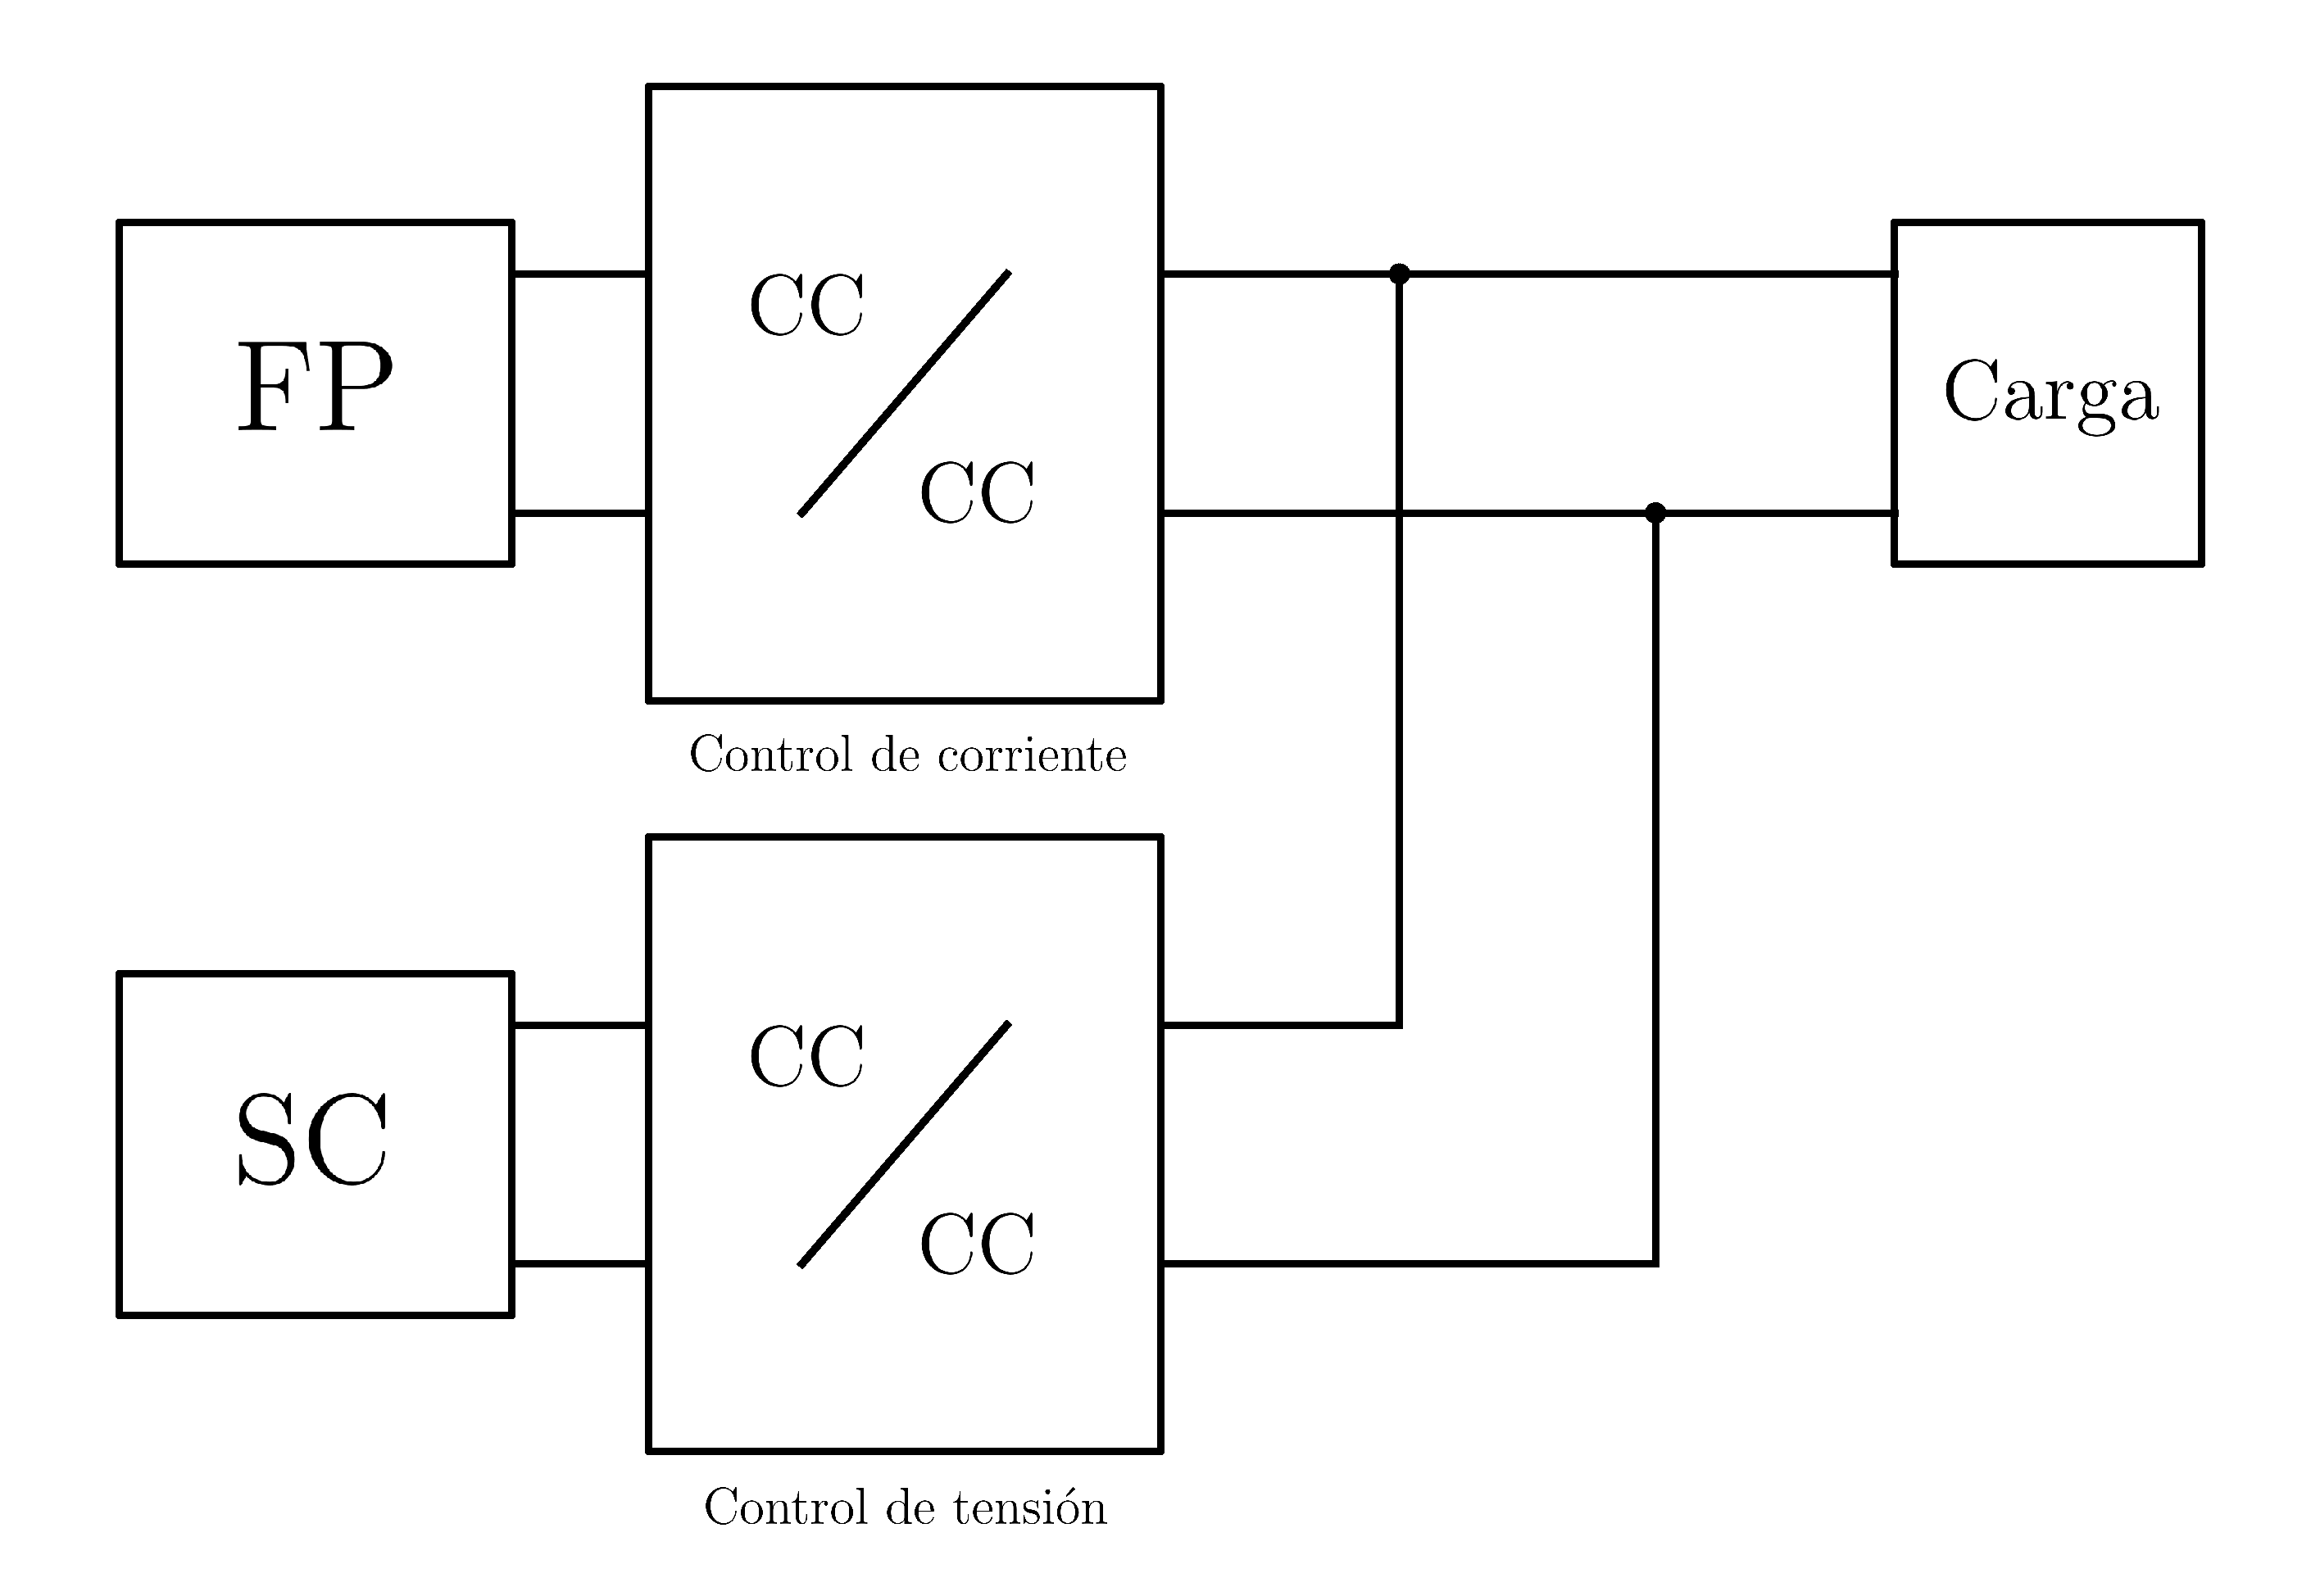
\includegraphics[width=0.55\columnwidth]{Imágenes/Ensayos/Con módulos de almacenamiento/Supercapacitores/Con fuente de potencia/Diagrama del ensayo.pdf}
  \caption{Diagrama del sistema con fuente de potencia y banco de supercapacitores.}
  \label{esquema-fp-sc}
\end{figure}

Utilizando un convertidor CC-CC para cada elemento de alimentación permite un control más versátil del sistema. Para esta configuración, el objetivo es el mismo que el ensayo desarrollado en la Sección \ref{sc-como-alimentacion}, con el banco de supercapacitores entregando el pico de demanda y la fuente de potencia proveyendo la potencia media. 

Con este fin, el convertidor que se encuentra del lado del bus de continua y corresponde al banco de supercapacitores presenta el sistema de control de tensión diseñado en el Capítulo \ref{diseno-control}, mientras que el convertidor de la fuente de potencia debe mantener el nivel de tensión en los supercapacitores que establezca su referencia, y procurar que la fuente entregue la corriente media que requiera la carga (es decir, que el banco de supercapacitores entregue una corriente media nula). La acción de control planteada para este último convertidor consistió de un lazo de control de corriente con una referencia que tenga a ambos elementos en consideración:

\begin{equation}
  i_{{FP}_{ref}} = K_1 \, \int_{0}^{t} i_{SC} \, dt + K_2 \, \int_{0}^{t} (V_{{SC}_{ref}} - v_{SC}) \, dt
\end{equation}

En donde ambas constantes $K_1$ y $K_2$ toman el valor de 10. Para este ensayo, el algoritmo de control fue implementado en otra placa de desarrollo, llamada DE10-Lite Board\textsuperscript\textregistered\hspace{0.6pt} de Terasic, la cual está basada en la FPGA MAX 10 de Altera (ahora Intel). 

Esta placa fue utilizada debido a que dispone de un conversor analógico-digital de 6 canales multiplexados a \SI{1}{\mega\sample/\second}, lo que permite muestrear las cuatro variables necesarias para el sistema de control planteado a \SI{250}{\kilo\sample/\second}: la corriente de entrada del primer convertidor (corriente del banco de supercapacitores), la corriente de entrada del segundo convertidor (corriente de la fuente de potencia), la tensión de entrada del primer convertidor (la tensión del banco de supercapacitores), y finalmente la tensión de salida del primer convertidor (la tensión de carga).

En la Figura \ref{foto-ensayo} se observa la disposición del sistema eléctrico híbrido ensayado en el instituto. Los elementos presentes en este ensayo son:

\begin{enumerate}
  \item La fuente de potencia.
  \item El banco de supercapacitores junto a su módulo de seguridad.
  \item El convertidor electrónico de potencia CC-CC conectado a la fuente de potencia.
  \item El convertidor electrónico de potencia CC-CC conectado al banco de supercapacitores.
  \item Placa de desarrollo DE10-Lite Board.
  \item Los circuitos auxiliares de interconexión y descarga.
  \item Los capacitores de interconexión.
\end{enumerate}

\begin{figure}[hbt!]
  \centering
  \includegraphics[width=0.60\columnwidth]{Imágenes/Ensayos/Con módulos de almacenamiento/Supercapacitores/Con fuente de potencia/Foto de la configuración.pdf}
  \caption{Foto de la configuración del sistema híbrido eléctrico.}
  \label{foto-ensayo}
\end{figure}

El primer ensayo del sistema consistió en la carga del banco de supercapacitores a \SI{12}{\volt}, para luego realizar pequeños escalones de unitarios de la tensión de bus, de \SI{16}{\volt} a \SI{24}{\volt}. Esta prueba fue realizada con una resistencia de carga \SI{40}{\ohm}, y una tensión de fuente de potencia de \SI{12}{\volt}.

En la Figura \ref{u-primer-ensayo-hibrido} pueden observarse las tensiones del banco y del bus. En la carga del banco, se observa una rampa positiva en la tensión de los supercapacitores y una corriente constante, esto último siendo producto del lazo interno de corriente de la fuente de potencia con una referencia manual para poder realizar una carga controlada. Luego, al activar la referencia automática del control de corriente de la fuente, se observa un pico inverso en la tensión de los supercapacitores. Debido al gran orden de magnitud temporal que posee este proceso, los supercapacitores no se llegan a cargar completamente, y por lo tanto en el ensayo no es posible apreciar cómo se establecen a la tensión de referencia. 

\begin{figure}[hbt!]
  \centering
  \subfloat[Tensiones de bus y del banco de supercapacitores.\label{u-primer-ensayo-hibrido}]{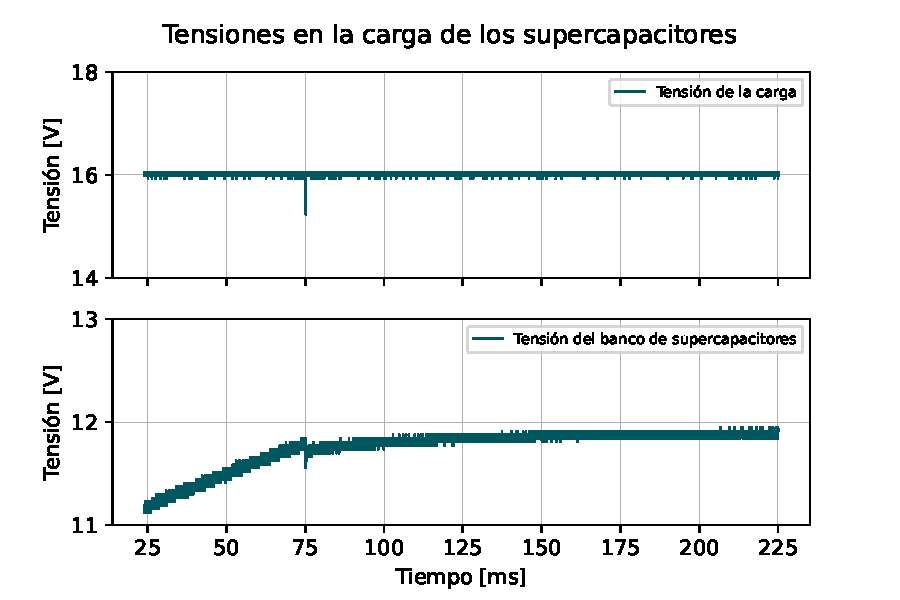
\includegraphics[width=0.45\textwidth]{Imágenes/Ensayos/Con módulos de almacenamiento/Supercapacitores/Con fuente de potencia/Primer ensayo/Tensiones en carga de los supercapacitores.pdf}}    
  \subfloat[Corrientes de fuente de potencia y del banco.\label{i-primer-ensayo-hibrido}]{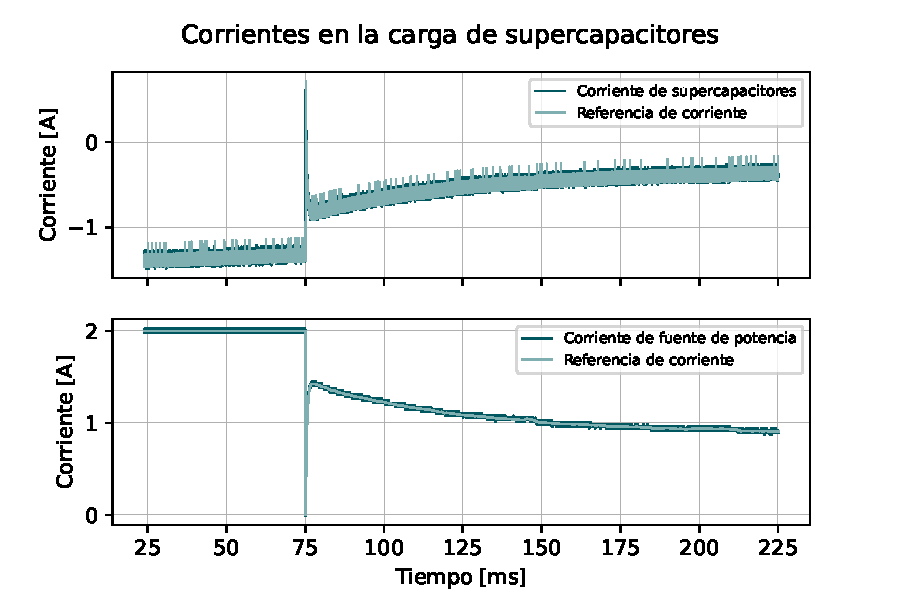
\includegraphics[width=0.45\textwidth]{Imágenes/Ensayos/Con módulos de almacenamiento/Supercapacitores/Con fuente de potencia/Primer ensayo/Corrientes en la carga de supercapacitores.pdf}}
  \caption{Tensiones y corrientes en la carga del banco de supercapacitores.}
  \label{primer-ensayo-hibrido}
\end{figure}

Para entender con mayor claridad el proceso, en la Figura \ref{i-primer-ensayo-hibrido} se grafican las corrientes de ambos módulos. Aquí se puede observar al principio cómo la fuente de potencia entrega corriente de forma constante, y una vez habilitado el control automático, la corriente disminuye lentamente mientras los supercapacitores se cargan, debido a la acción de control dependiente de la tensión del banco.

Una vez que el proceso de carga es finalizado, se efectúan los escalones de la tensión de bus. Se puede visualizar en la Figura \ref{u-2-primer-ensayo-hibrido} como la tensión del bus sigue en cuestión de milisegundos a la referencia, y cómo se genera un pequeño pico inverso en la tensión de los supercapacitores en cada salto, lo cual representa la entrega de potencia instantánea que demanda el bus al aumentar su tensión.

\begin{figure}[hbt!]
  \centering
  \subfloat[Tensiones de bus y del banco de supercapacitores.\label{u-2-primer-ensayo-hibrido}]{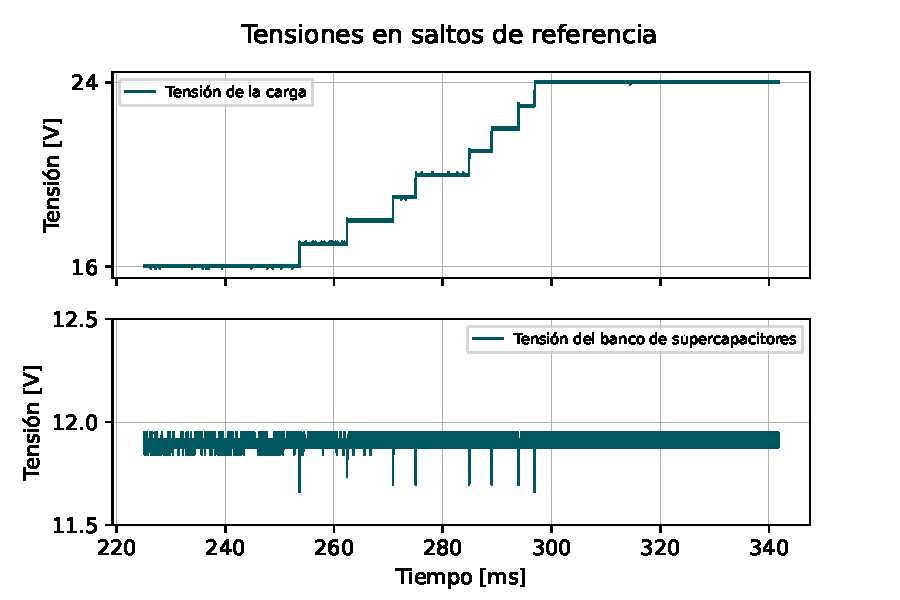
\includegraphics[width=0.45\textwidth]{Imágenes/Ensayos/Con módulos de almacenamiento/Supercapacitores/Con fuente de potencia/Primer ensayo/Tensiones en saltos de referencia.pdf}}    
  \subfloat[Corrientes de fuente de potencia y del banco.\label{i-2-primer-ensayo-hibrido}]{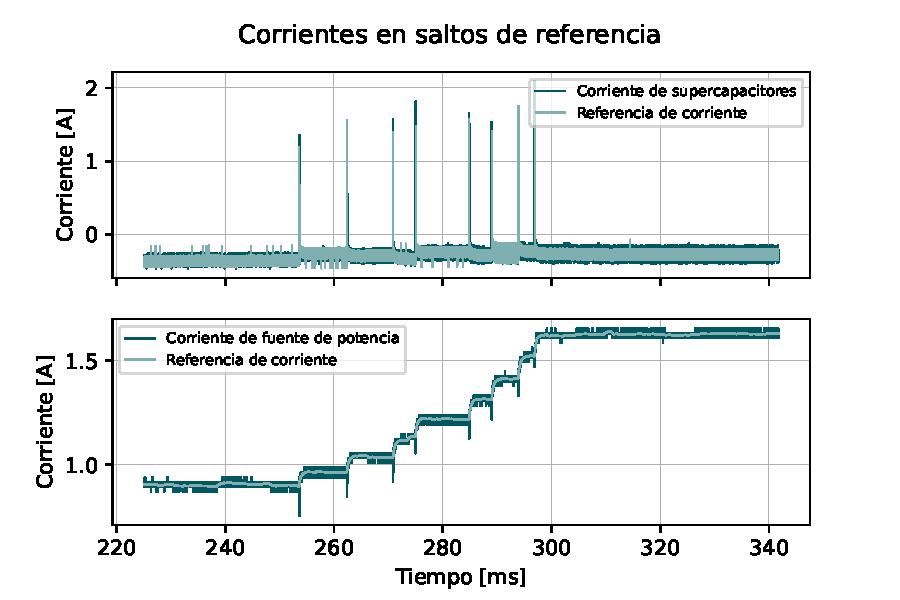
\includegraphics[width=0.45\textwidth]{Imágenes/Ensayos/Con módulos de almacenamiento/Supercapacitores/Con fuente de potencia/Primer ensayo/Corrientes en saltos de referencia.pdf}}
  \caption{Tensiones y corrientes en la carga del banco de supercapacitores.}
  \label{primer-ensayo-hibrido-2}
\end{figure}

Este pico inverso es visible con mayor facilidad en la corriente de los supercapacitores en la Figura \ref{i-2-primer-ensayo-hibrido}, mientras que se observa una respuesta escalonada más suave en la corriente de la fuente de potencia, similar a la tensión de carga. Ya establecida la tensión de carga en \SI{24}{\volt}, se procede con el segundo ensayo, el cual consistió en la variación de la resistencia de carga para observar la dinámica del sistema híbrido eléctrico.

\begin{figure}[hbt!]
  \centering
  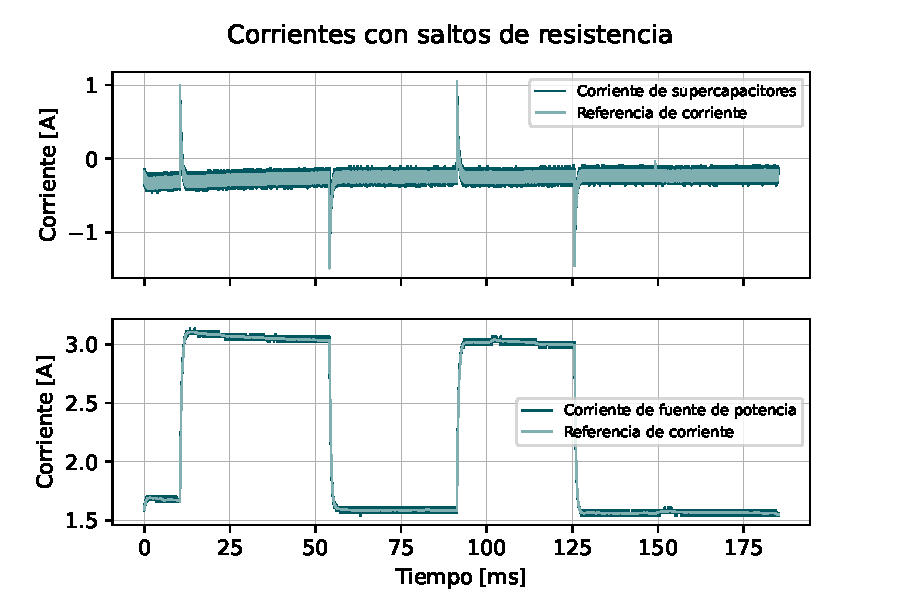
\includegraphics[width=0.53\columnwidth]{Imágenes/Ensayos/Con módulos de almacenamiento/Supercapacitores/Con fuente de potencia/Segundo ensayo/Corrientes con saltos de resistencia.pdf}
  \caption{Corrientes de fuente de potencia y del banco con saltos de resistencia de carga.}
  \label{i-segundo-ensayo-hibrido}
\end{figure}

En la Figura \ref{i-segundo-ensayo-hibrido} se aprecia claramente la dinámica esperada para este sistema. En un salto positivo de resistencia, se observa cómo se genera un pico de corriente de los supercapacitores para luego establecerse en cero, lo cual se traduce a una entrega instantánea de la potencia demandada por la variación de la carga. A su vez, la corriente de la fuente de potencia presenta un lento crecimiento para después establecerse en la corriente media necesaria para que la tensión de carga alcance a la tensión de referencia.

La Figura \ref{u-segundo-ensayo-hibrido} presenta pequeños pulsos que se corresponden con las variaciones de la resistencia de carga. Estas variaciones del orden de los \SI{}{\milli\volt} en la tensión del banco de supercapacitores equivalen a una pequeña descarga o carga del banco ante un salto de \SI{20}{\ohm} a \SI{40}{\ohm} o viceversa, lo que significa que no toda la capacidad de carga del arreglo de supercapacitores es aprovechada. Por lo tanto, es posible utilizar un banco con menor capacidad para este sistema híbrido. A lo largo de este ensayo se corrobora el control constante de la tensión de carga a \SI{24}{\volt}.

\begin{figure}[hbt!]
  \centering
  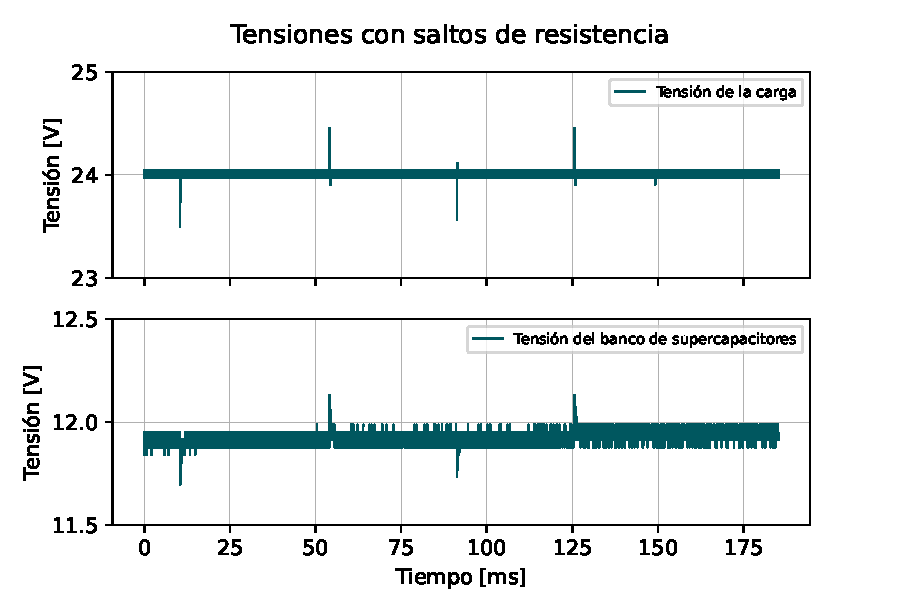
\includegraphics[width=0.53\columnwidth]{Imágenes/Ensayos/Con módulos de almacenamiento/Supercapacitores/Con fuente de potencia/Segundo ensayo/Tensiones con saltos de resistencia.pdf}
  \caption{Tensiones de fuente de potencia y del banco con saltos de resistencia de carga.}
  \label{u-segundo-ensayo-hibrido}
\end{figure}

El último ensayo realizado con esta topología del sistema híbrido, y bajo el marco de este proyecto, consistió de la variación de la tensión del banco de supercapacitores de \SI{12}{\volt} a \SI{13}{\volt}, un escalón de resistencia de \SI{40}{\ohm} a \SI{10}{\ohm}, luego un salto negativo unitario de la tensión del banco nuevamente a \SI{12}{\volt}, y finalmente otro escalón de resistencia \SI{10}{\ohm} a \SI{40}{\ohm}.

\begin{figure}[hbt!]
  \centering
  \subfloat[Tensiones de fuente de potencia y del banco.\label{u-tercer-ensayo-hibrido}]{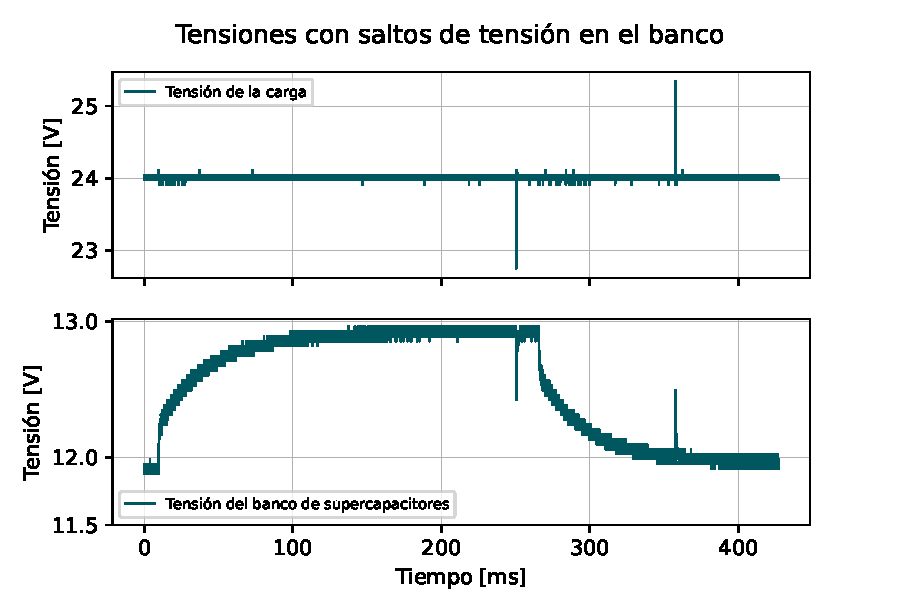
\includegraphics[width=0.45\textwidth]{Imágenes/Ensayos/Con módulos de almacenamiento/Supercapacitores/Con fuente de potencia/Tercer ensayo/Tensiones con saltos de tensión en el banco.pdf}}    
  \subfloat[Corrientes de fuente de potencia y del banco.\label{i-tercer-ensayo-hibrido}]{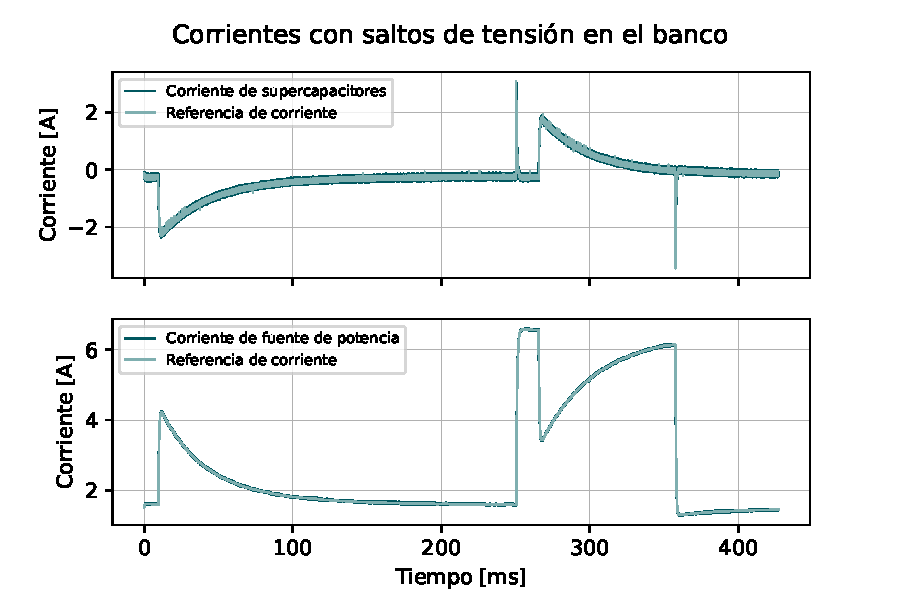
\includegraphics[width=0.45\textwidth]{Imágenes/Ensayos/Con módulos de almacenamiento/Supercapacitores/Con fuente de potencia/Tercer ensayo/Corrientes con saltos de tensión en el banco.pdf}}
  \caption{Formas de onda con variaciones de tensión de banco y resistencia de carga.}
  \label{tercer-ensayo-hibrido}
\end{figure}

En la Figura \ref{u-tercer-ensayo-hibrido} se presentan nuevamente la tensión de los supercapacitores y la del bus. Cuando se efectúa el salto de \SI{12}{\volt} a \SI{13}{\volt}, puede observarse un transitorio del orden de cientos de segundos hasta el establecimiento al nuevo nivel de tensión del banco, y un pulso negativo en las tensiones, causado por un salto de \SI{40}{\ohm} a \SI{10}{\ohm} de la resistencia de carga. Esta dinámica lenta es deseable, ya que la recarga y descarga del banco de supercapacitores debe ser más lenta que las dinámicas de tensión del bus, para asegurar que no se sobrecargue a la fuente principal. Restableciendo la referencia en \SI{12}{\volt}, la tensión nuevamente vuelve a su valor original con un comportamiento exponencial negativo. El pico de tensión observado es debido al salto positivo de la carga de \SI{10}{\ohm} a \SI{40}{\ohm}. A lo largo de este ensayo, la tensión de bus se mantiene constante en \SI{24}{\volt} con perturbaciones ante los cambios de resistencia de carga.

Como la dinámica de las corrientes es mucho más rápida que la de las tensiones, en la Figura \ref{i-tercer-ensayo-hibrido} la corriente de la fuente de potencia reacciona rápidamente ante el cambio de referencia de la tensión del banco, alcanzando un valor mayor a \SI{4}{\ampere} para luego establecerse nuevamente en la corriente necesaria para mantener el bus a \SI{24}{\volt}.

Luego del establecimiento de la corriente, se produce el salto negativo de resistencia de carga, lo que significa que la fuente de potencia debe entregar más corriente para mantener el valor de tensión de bus en \SI{24}{\volt}. Este escalón de demanda es visible aproximadamente a partir del segundo 250. 

Un breve tiempo después, la referencia de tensión del banco se vuelve a fijar en \SI{12}{\volt}, lo que produce una reacción en la corriente de la fuente de potencia generando un pico inverso para disminuir su entrega de energía y permitir que los supercapacitores disminuyan su nivel de tensión a \SI{12}{\volt}. Por último, se realiza un escalón positivo de resistencia de carga de \SI{10}{\ohm} a \SI{40}{\ohm}, lo que reduce a la corriente entregada por la fuente de potencia y la corriente del banco.


\section{Resumen}

En este capítulo se presenta la etapa final del proyecto, con los ensayos de distintos tipos de configuraciones del sistema eléctrico híbrido y el observamiento de su comportamiento mediante distintos tipos de perturbaciones y situaciones de operación. 

A partir de un proceso progresivo se pudo verificar cómo los componentes individuales funcionaban correctamente, para luego empezar a ensayar al sistema de control en su enteridad a partir del control de tensión y corriente.

Este sistema de control fue implementado para distintas topologías del sistema eléctrico híbrido, ubicando a los módulos de almacenamiento como fuentes de energía y como carga para observar la dinámica que presentan en cada configuración.

La última topología del sistema híbrido eléctrico demostró cómo el banco de supercapacitores es capaz de entregar un pulso instantáneo de energía mientras la fuente de potencia es la que proveé la corriente media que demanda la carga.

\newpage